\documentclass{ximera}

\newcommand{\dfn}{\textbf}
\renewcommand{\vec}[1]{{\overset{\boldsymbol{\rightharpoonup}}{\mathbf{#1}}}\hspace{0in}}
%% Simple horiz vectors
\renewcommand{\vector}[1]{\left\langle #1\right\rangle}
\newcommand{\arrowvec}[1]{{\overset{\rightharpoonup}{#1}}}
\newcommand{\R}{\mathbb{R}}
\newcommand{\transpose}{\intercal}
\newcommand{\ro}{\texttt{R}}%% row operation
\newcommand{\dotp}{\bullet}%% dot product

\usetikzlibrary{calc,bending}
\tikzset{>=stealth}


\usepackage{mdframed} % For framing content
%\usepackage{ifthen}   % For conditional statements

% Define the 'concept' environment with an optional header
\newenvironment{concept}[1][]{%
  \begin{mdframed}[linecolor=black, linewidth=2pt, innertopmargin=5pt, innerbottommargin=5pt, skipabove=12pt, skipbelow=12pt]%
    \noindent\large\textbf{#1}\normalsize%
}{%
  \end{mdframed}%
}











%% \colorlet{textColor}{black}
%% \colorlet{background}{white}
%% \colorlet{penColor}{blue!50!black} % Color of a curve in a plot
%% \colorlet{penColor2}{red!50!black}% Color of a curve in a plot
%% \colorlet{penColor3}{red!50!blue} % Color of a curve in a plot
%% \colorlet{penColor4}{green!50!black} % Color of a curve in a plot
%% \colorlet{penColor5}{orange!80!black} % Color of a curve in a plot
%% \colorlet{penColor6}{yellow!70!black} % Color of a curve in a plot
%% \colorlet{fill1}{penColor!20} % Color of fill in a plot
%% \colorlet{fill2}{penColor2!20} % Color of fill in a plot
%% \colorlet{fillp}{fill1} % Color of positive area
%% \colorlet{filln}{penColor2!20} % Color of negative area
%% \colorlet{fill3}{penColor3!20} % Fill
%% \colorlet{fill4}{penColor4!20} % Fill
%% \colorlet{fill5}{penColor5!20} % Fill
%% \colorlet{gridColor}{gray!50} % Color of grid in a plot

\usetikzlibrary{matrix}
\author{Parisa Fatheddin \and Bart Snapp}

%% Jim Hefferon’s Linear Algebra. (CC-BY-NC-SA)
%% Anna Davis and Paul Zachlin: https://github.com/annadavismath/LinearAlgebraV2
%% https://ximera.osu.edu/linearalgebrav3/LinearAlgebraInteractiveIntro/SYS-0030/main

%% https://www.cis.upenn.edu/~cis6100/Notices-06-11-Gausselim.pdf
%% https://www.sciencedirect.com/science/article/pii/S0315086010000376


\title{Matrices and systems of linear equations}




\begin{document}
\begin{abstract}
  We use matrices to solve systems of linear equations.
\end{abstract}
\maketitle

Gaussian elimination is technique for solving systems of linear
equations. It is (obviously) named after
\link[Gauss]{https://en.wikipedia.org/wiki/Carl_Friedrich_Gauss}
($1799$--$1855$). However, it was known to
\link[Legendre]{https://en.wikipedia.org/wiki/Adrien-Marie_Legendre}
($1752$--$1833$) and even
\link[Euler]{https://en.wikipedia.org/wiki/Leonhard_Euler}
($1707$--$1783$) before him. Moreover, it seems that these \textit{legends of
mathematics} did not think highly of the method: Gauss refereed to it
as ``common;'' Legendre called it ``ordinary;'' Euler ``did not
recommend'' this method to students.




Despite this inauspicious start, \textbf{Gaussian elimination is a
  tremendously important technique today.} It reduces a problem to
its barest components, and gives a method, an algorithm, that can be
programmed into a computer that will solve systems of linear
equations. Our mathematical heroes' disdain for this method is a
consequence of the fact that \textit{not even they could have dreamt of the awesome
computational power of modern computers.}



\section{Row operations on matrices}


Any time we have a \dfn{system of equations} we may represent it with a
\dfn{matrix}
\[
\begin{array}{ccccccc}
       & & 3y &-& 3z &=& -3 \\
     x& +&3y&-&3z&=&2\\
     -3x& -&9y&-&11z&=&0
\end{array}
\qquad\Longrightarrow\qquad
\left(\begin{array}{ccc|c}
  0 &   3 & -3 & -3 \\
  1 &   3 & -3 & 2  \\
  -3& -9  & 11 & 0
\end{array}\right).
\]
This is an example of a matrix used to store data. Some folks call
this an \dfn{augmented matrix}, and they write stuff like this:
\[
A = \underbrace{\begin{pmatrix}
  0 & 3 & -3  \\
  1 &  3  & -3 \\
 -3 & -9 & 11
\end{pmatrix}}_{\text{the coefficients}},
\quad
B =
\underbrace{\begin{pmatrix}
 -3\\ 2 \\ 0 
\end{pmatrix}}_{\text{right-hand side}},
\quad
\left(A|B\right) = \underbrace{\left(\begin{array}{ccc|c}
  0 &   3 & -3 & -3 \\
  1 &   3 & -3 & 2  \\
  -3& -9  & 11 & 0
\end{array}\right)}_{\text{augmented matrix}}.
\]

\begin{question}
  Consider the following system of equations:

  Write the augmented matrix for this system of equations.
  \begin{prompt}
    \[
    \left(\begin{array}{ccc|c}
      \answer{} & \answer{} & \answer{} & \answer{}
    \end{array}\right)
    \]
  \end{prompt}
\end{question}

We are going to use matrices to solve this system of equations. The
method we describe below is often called \dfn{Gaussian elimination}
or simply \dfn{elimination}. To do this, we're going to introduce
\dfn{row operations}. The row operations will allow us to change the
form of the matrix \emph{without changing the solutions}. The idea is
this we start with a big matrix,
\[
\begin{pmatrix}
  \bullet & \bullet & \bullet & \bullet \\
  \bullet & \bullet & \bullet & \bullet \\
  \bullet & \bullet & \bullet & \bullet 
\end{pmatrix}
\quad
\Rightarrow
\quad
\begin{pmatrix}
  \bullet & \bullet & \bullet & \bullet \\
     0   & \bullet & \bullet & \bullet \\
     0  &    0 & \bullet & \bullet 
\end{pmatrix}
\quad
\Rightarrow
\quad
\begin{pmatrix}
  1 & 0 & 0  & \bullet \\
     0   & 1  &  0 & \bullet \\
     0  &    0 & 1 & \bullet 
\end{pmatrix}
\]
and transform it into a form where we can simply ``read-off'' the
information about the system of equations, including the solutions.  We
discuss the row operations that allow such a transformation below.



\subsection{Swapping two rows} Since swapping the order of the equations in a
  system of equations does not change the solutions, we may swap rows
  in an augmented matrix. We denote swapping the $i$th row with the
  $j$th row by $R_i\leftrightarrow R_j$. As an example, we can swap
  the first and second rows of the matrix below:
 \[
\left(\begin{array}{ccc|c}
  0 &   3 & -3 & -3 \\
  1 &   3 & -3 & 2  \\
  -3& -9  & 11 & 0
\end{array}\right)
\qquad
\begin{array}{c}
  R_1\leftrightarrow R_2\\\Longrightarrow
\end{array}
\qquad
\left(\begin{array}{ccc|c}
  1 &   3 & -3 & 2  \\
  0 &   3 & -3 & -3 \\
  -3& -9  & 11 & 0
\end{array}\right)
\]

\begin{question}
\end{question}

  
\subsection{Multiply by a nonzero constant and add different rows} 
We may multiply equations by nonzero constants and add equations together
\emph{without affecting the solution.} Hence we may multiply the first
row by $3$ and add it to the third row, storing the answer in the
third row (you could have chosen either of the summands).
\[
\left(\begin{array}{ccc|c}
  1 &   3 & -3 & 2  \\
  0 &   3 & -3 & -3 \\
  -3& -9  & 11 & 0
\end{array}\right)
\qquad
\begin{array}{c}
  3R_1+R_3\rightarrow R_3\\\Longrightarrow
\end{array}
\qquad
\left(\begin{array}{ccc|c}
  1 &   3 & -3 & 2  \\
  0 &   3 & -3 & -3 \\
  0& 0  & 2 & 6
\end{array}\right).
\]

\begin{question}
\end{question}



At this point, we should draw your attention to the \emph{form} of the matrix. This matrix

\[
\begin{pmatrix}
  1 &   3 & -3 & 2  \\
  0 &   3 & -3 & -3 \\
  0& 0  & 2 & 6
\end{pmatrix}
\qquad
\text{is of this form:}
\qquad
\begin{pmatrix}
  \bullet & \bullet & \bullet & \bullet \\
     0   & \bullet & \bullet & \bullet \\
     0  &    0 & \bullet & \bullet 
\end{pmatrix}
\]



We'll discuss the implications of this form below.


\section{Row echelon form}

We can write many different matrices that all represent systems
of equations that have a common solution. For example:
\[
\begin{pmatrix}
 0 &   3 & -3 & -3 \\
  1 &   3 & -3 & 2  \\
  -3& -9  & 11 & 0
\end{pmatrix},
\quad
\begin{pmatrix}
  1 &   3 & -3 & 2  \\
  0 &   3 & -3 & -3 \\
  -3& -9  & 11 & 0
\end{pmatrix},
\quad
\begin{pmatrix}
  1 &   3 & -3 & 2  \\
  0 &   3 & -3 & -3 \\
  0& 0  & 2 & 6
\end{pmatrix},
\]
are all different matrices representing the same solution to the
system of equations:
\[
\begin{array}{ccccccc}
       & & 3y &-& 3z &=& 2 \\
     x& +&3y&-&3z&=&-3\\
     -3x& -&9y&-&11z&=&0
\end{array}
\]
Some `forms' of these matrices are more convenient than others. One
useful form is called \dfn{row echelon form} or \dfn{triangular
  form}. An \textit{echelon} is a military term meaning a formation
(of soldiers, vehicles, and so on) that makes a ``stair step''
shape. All of the matrices below are in row echelon form:
\begin{center}
\begin{tikzpicture}
  \draw[line width=1.3em,black!15!white] (-1.9,.455) -- (1.8,.455);
  \draw[line width=1.3em,black!15!white] (-.8,.025) -- (1.8,.025);
  \draw[line width=1.3em,black!15!white] (.7,-.42) -- (1.8,-.42);
\node at (0,0) {$\begin{pmatrix}
 ~1~&2&-1&-5&0&~2~\\0&0&3&0&2&0\\0&0&0&0&1&0
  \end{pmatrix},$};
%\draw (-1.9,.7) -- (-1.9,.25) -- (-.8,.25) -- (-.8, -.2) -- (.7,-.2) -- (.7,-.7);
\end{tikzpicture}
\quad\begin{tikzpicture}
  \draw[line width=13pt,black!15!white] (-.6,.455) -- (.45,.455);
  \draw[line width=13pt,black!15!white] (-.05,.025) -- (.45,.025);
\node at (0,0) {$\begin{pmatrix}
 ~4~&~0~\\0&1\\0&0
  \end{pmatrix},$};
%\draw (-.6,.7) -- (-.6,.25) -- (-.05,.25) -- (-.05, -.2) -- (.45,-.2) -- (.45,-.7);
\end{tikzpicture}
\quad
\begin{tikzpicture}
  \draw[line width=1.3em,black!15!white] (-1.5,.455) -- (1.35,.455);
  \draw[line width=1.3em,black!15!white] (-1,.025) -- (1.35,.025);
  \draw[line width=1.3em,black!15!white] (-.4,-.42) -- (1.35,-.42);
\node at (0,0) {$\begin{pmatrix}
  ~1~ &   3 & -3 & ~2~  \\
  0 &   3 & -3 & ~-3~ \\
  0& 0  & 2 & 6
  \end{pmatrix}.$};
%\draw (-1.5,.7) -- (-1.5,.25) -- (-1,.25) -- (-1, -.2) -- (-.4,-.2) -- (-.4,-.7);
\end{tikzpicture}
\end{center}
We've highlighted the \textit{echelon} pattern in each of the matrices
above. Now let's give a definition.

\begin{definition}
We say a matrix $M$ is in \dfn{row echelon form} if every nonzero row
contains a nonzero entry $M_{i,j}\ne 0$ such that
\begin{itemize}
\item Every entry below $M_{i,j}$ is zero, $M_{k,\l}=0$ whenever $k> i$.
\item Every entry to the left of $M_{i,j}$ is zero, $M_{k,\l}=0$ whenever $\l < j$.
\end{itemize}
Such an $M_{i,j}$ is called a \dfn{pivot} of $M$.
\end{definition}

\begin{question}
  id in REF and id pivots
\end{question}



\subsection{How does row echelon form help?}

Let's think about our original system of equations. We've shown that
this corresponds to a matrix in row echelon from:
\[
\begin{array}{ccccccc}
       & & 3y &-& 3z &=& 2 \\
     x& +&3y&-&3z&=&-3\\
     -3x& -&9y&-&11z&=&0
\end{array}
\qquad\Longrightarrow\qquad
\begin{pmatrix}
  1 &   3 & -3 & 2  \\
  0 &   3 & -3 & -3 \\
  0& 0  & 2 & 6
\end{pmatrix}
\]
But this final matrix that we obtained from row operations, (directly)
corresponds to the following system of equations:
\[
\left(\begin{array}{ccc|c}
  1 &   3 & -3 & 2  \\
  0 &   3 & -3 & -3 \\
  0& 0  & 2 & 6
\end{array}\right)
\qquad\Longrightarrow\qquad
\begin{array}{ccccccc}
     x  &+ & 3y &-& 3z &=& 2 \\
     &  &3y&-&3z&=&-3\\
     & & & &2z&=&6
\end{array}
\]



\begin{algorithm}[Row Echelon Form (REF)]
  Here we explain a general algorithm for reducing a matrix to row
  echelon form in plain terms.
  \begin{enumerate}
  \item Determine the leftmost column containing a nonzero entry (it exists if the matrix is nonzero).
  \item Use row operations so that the first nonzero column has a non-zero entry in the first row.
  \item Use row operations to make the entries below this nonzero entry equal to zero.
  \item Repeat the previous four steps on the submatrix consisting of
    all except the first row, until reaching the end of the rows.
  \end{enumerate}
\end{algorithm}

Pictorially, we can imagine this algorithm working as follows:

\[
\begin{pmatrix}
  \bullet & \bullet & \bullet & \bullet \\
  \bullet & \bullet & \bullet & \bullet \\
  \bullet & \bullet & \bullet & \bullet 
\end{pmatrix}
\Rightarrow
\begin{pmatrix}
  \bullet & \bullet & \bullet & \bullet \\
  0       & \bullet & \bullet & \bullet \\
  0       & \bullet & \bullet & \bullet 
\end{pmatrix}
\]

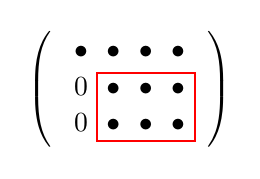
\begin{tikzpicture}
  \matrix (m) [matrix of math nodes,left delimiter={(},right delimiter={)}] {
    \bullet & \bullet & \bullet & \bullet \\
    0       & \bullet & \bullet & \bullet \\
    0       & \bullet & \bullet & \bullet \\
  };

  % Draw the rectangle around the submatrix
  \draw[red,thick] (m-2-2.north west) rectangle (m-3-4.south east);

\end{tikzpicture}



















\section{Reduced row echelon form}


Now comes the \emph{elimination} part of Gaussian elimination. 

\section{Putting it all together}


\begin{example}
  Solve for $x$, $y$, and $z$ in the following system of equations:
  \begin{align*}
    2x + 3y + z  &= 5 \\
    x -2y+ 2z &=-9\\
    3x +y- 3z &=14
  \end{align*}

\begin{solution}
First we'll represent this as an agumented matrix.
\[
\left(\begin{array}{ccc|c}
  2 & 3 & 1 & 5 \\
  1 &  -2 & 2 &-9 \\
  3 &  1 & -3 & 14
\end{array}\right)
\]
Our first goal is to convert our matrix to row echelon form. Noting
that changing the order of equations does not affect the solutions of the system
\[
\left(\begin{array}{ccc|c}
  2 & 3 & 1 & 5 \\
  1 &  -2 & 2 &-9 \\
  3 &  1 & -3 & 14
\end{array}\right)
\begin{array}{c}
  R_1\leftrightarrow R_2\\\Longrightarrow
\end{array}
\left(\begin{array}{ccc|c}
  1 &  -2 & 2 &-9 \\
  2 & 3 & 1 & 5 \\
  3 &  1 & -3 & 14
\end{array}\right),
\]
Note that changing the order of equations does not affect the system
and it is the same as interchanging rows in the matrix, denoted as
$R_1 \leftrightarrow R_2$. By addition method we proceed by
multiplying the first equation by $-2$ and adding it to the second
equation. Afterwards, we multiply the first equation by $-3$ and add
it to the third equation:
\[
\begin{array}{ccccccccc}
     (-2)&&(x& -&2y&+&2z&=&-9)\\
     +&& 2x &+& 3y &+& z &=& 5 \\
     &&-&-&-&-&-&-&-\\
     \Rightarrow&& & &7y&-&3z&=&23
\end{array}
\hspace{.2cm}\Rightarrow \hspace{.2cm}
\left(\begin{array}{ccc|c}
  1 &  -2 & 2 &-9 \\
  0 & 7 & -3 & 23 \\
  3 &  1 & -3 & 14
\end{array}\right),
\]
and
\[
\begin{array}{ccccccccc}
     (-3)&&(x& -&2y&+&2z&=&-9)\\
     +&& 3x &+& y &-& 3z &=& 14 \\
     &&-&-&-&-&-&-&-\\
     \Rightarrow&& & &7y&-&9z&=&41
\end{array}
\hspace{.2cm}\Rightarrow \hspace{.2cm}
\left(\begin{array}{ccc|c}
  1 &  -2 & 2 &-9 \\
  0 & 7 & -3 & 23 \\
  0 &  7 & -9 & 41
\end{array}\right).
\]
The above operations can be written in condensed form as $-2R_1 + R_2$ and $-3R_1 + R_3$, respectively. Observe that the row that is multiplied by a number does not change. For example, the first row above stayed the same and the row that it was added to changed. It is convenient to multiply each entry of row one by the appropriate number and write it above the row as side work and erase the numbers after adding them to the other row. It is important not to change the row itself. \\
Now we see that both $y$ variables have $7$ as the coefficient. Thus, the best way to proceed is to eliminate the $y$ variable:
\[
\begin{array}{ccccccc}
     (-1)&&(7y&-&3z&=&23)\\
     +&& 7y &-& 9z &=& 41 \\
     &&-&-&-&-&-\\
     \Rightarrow&& &-&6z&=&18
\end{array}
\hspace{.2cm}\Rightarrow \hspace{.2cm}
\left(\begin{array}{ccc|c}
  1 &  -2 & 2 &-9 \\
  0 & 7 & -3 & 23 \\
  0 &  0 & -6 & 18
\end{array}\right).
\]
It is now natural to solve for $z$ and obtain:
\[
\begin{array}{ccc}
     &&z = -3\\
     \text{ also } &&7y- 3z=23  \hspace{.3cm}\Rightarrow\hspace{.3cm} y- \frac{3}{7}z = \frac{23}{7}
\end{array}
\hspace{.2cm}\Rightarrow \hspace{.2cm}
\left(\begin{array}{ccc|c}
  1 &  -2 & 2 &-9 \\
  0 & 1 & -3/7 & 23/7 \\
  0 &  0 & 1 & -3
\end{array}\right),
\]
where the operations translate to $R_{3}/(-6)$ and $R_{2}/7$, respectively. By substitution, we obtain,\\

\hspace{.5cm} $z = -3   \hspace{.5cm}\Rightarrow \hspace{.5cm} y- \frac{3}{7}(-3) = \frac{23}{7} \hspace{.5cm}\Rightarrow \hspace{.5cm} y= \frac{23-9}{7}= 2,$
\\ \\ \hspace{.5cm} then putting $y$ and $z$ in the first equation gives $x -2(2)+2(-3)=-9$ from which we obtain, $x= 1$.

The same process may be applied to matrices by converting the rows back to equations and then using substitution. The matrix we obtained in which the diagonal entries are 1 and every entry below them is zero is said to be in row-echelon form. If one also makes the entries above the diagonal to become zero then the matrix is said to be in reduced row-echelon form. In example above, we may first make the entry above entry $a_{22}$ be zero:
\[
\left(\begin{array}{ccc|c}
  1 &  -2 & 2 &-9 \\
  0 & 1 & -3/7 & 23/7 \\
  0 &  0 & 1 & -3
\end{array}\right)
\hspace{.2cm}\xrightarrow{2R_{2}+R_{1}} \hspace{.2cm}
\left(\begin{array}{ccc|c}
  1 &  0 & 8/7 &-17/7 \\
  0 & 1 & -3/7 & 23/7 \\
  0 &  0 & 1 & -3
\end{array}\right),
\]
Then we use the 1 in row three to make the entries above it zero:
\[
\left(\begin{array}{ccc|c}
  1 &  0 & 8/7 &-17/7 \\
  0 & 1 & -3/7 & 23/7 \\
  0 &  0 & 1 & -3
\end{array}\right)
\hspace{.2cm}\xrightarrow[(3/7)R_{3}+R_{2}]{(-8/7)R_{3}+R_{1}} \hspace{.2cm}
\left(\begin{array}{ccc|c}
  1 &  0 & 0 &1 \\
  0 & 1 & 0& 2 \\
  0 &  0 & 1 & -3
\end{array}\right),
\]
which automatically leads to $z=-3$ and $y=2$ and $x=1$.
\end{solution}
\end{example}


\begin{example}
  There are two special cases that may occur in solving systems: the system may have no real solutions and the other is it can have infinitely many solutions. Here we discuss these two cases by going through examples.\\
Let us study at the following system,
\begin{eqnarray}\label{system}
\frac{2}{5}x + \frac{3}{10} y &=& 8\\
y -\frac{1}{4}w &=& 5\nonumber\\
\frac{3}{5}x + \frac{2}{5}z &=& 2\nonumber\\
6y - \frac{3}{2}w &=& -9.\nonumber
\end{eqnarray}
We write it in matrix form:
\[
\left(\begin{array}{ccccc|c}
   \answer[given]{2/5}&  \answer[given]{3/10} & \answer[given]{0} &\answer[given]{0} &8 \\
  \answer[given]{0}&  \answer[given]{1} & \answer[given]{0} &\answer[given]{-1/4} &5\\
  \answer[given]{3/5}&  \answer[given]{0} & \answer[given]{2/5} &\answer[given]{0} &2\\
  \answer[given]{0}&  \answer[given]{6} & \answer[given]{0} &\answer[given]{-3/2} &-9
\end{array}\right)
\]
To avoid calculations involving fractions, we first convert such entries to integers by multiplying their rows by the common denominator of the fractions in that row. Then we obtain,
\[
\left(\begin{array}{ccccc|c}
   \answer[given]{4}&  \answer[given]{3} & \answer[given]{0} &\answer[given]{0} &80 \\
  \answer[given]{0}&  \answer[given]{4} & \answer[given]{0} &\answer[given]{-1} &20\\
  3&  \answer[given]{0} & \answer[given]{2} &\answer[given]{0} &\answer[given]{10}\\
  \answer[given]{0}&  \answer[given]{12} & \answer[given]{0} &\answer[given]{-3} &\answer[given]{-18}
\end{array}\right)
\]
Then,
\[
\hspace{.2cm}\xrightarrow[-3R_{1} + R_{\answer[given]{3}}]{\answer[given]{1/4}R_{1}}\hspace{.2cm}
\left(\begin{array}{ccccc|c}
   \answer[given]{1}&  \answer[given]{3/4} & \answer[given]{0} &\answer[given]{0} &\answer[given]{20} \\
  \answer[given]{0}&  \answer[given]{4} & \answer[given]{0} &\answer[given]{-1} &20\\
  \answer[given]{0}&  \answer[given]{-9/4} & \answer[given]{2} &\answer[given]{0} &-50\\
  \answer[given]{0}&  \answer[given]{12} & \answer[given]{0} &\answer[given]{-3} &\answer[given]{-18}
\end{array}\right)\\
\]
\[
\hspace{.2cm}\xrightarrow[-12 R_{2} + R_{\answer[given]{4}}]{\answer[given]{1/4}R_{2}}\hspace{.2cm}
\left(\begin{array}{ccccc|c}
   \answer[given]{1}&  \answer[given]{3/4} & \answer[given]{0} &\answer[given]{0} &\answer[given]{20} \\
  \answer[given]{0}&  \answer[given]{1} & \answer[given]{0} &\answer[given]{-1/4} &5\\
  \answer[given]{0}&  \answer[given]{-9/4} & \answer[given]{2} &\answer[given]{0} &-50\\
  \answer[given]{0}&  \answer[given]{0} & \answer[given]{0} &\answer[given]{0} &\answer[given]{-78}
\end{array}\right)
\]
Thus, the last row translates to $0x+0y+0z+0w=-78$, that is $0=-78$, which can never be true. This means that the system has no solution. There is no $(x,y,z,w)$ that makes every equation in the system hold true. \\
Now let us consider the same system \eqref{system} with the second equation replaced with,
\begin{equation*}
y- \frac{1}{4}w= -\frac{3}{2}.
\end{equation*}
Then, the same steps may be followed as above to obtain,
\[
\left(\begin{array}{ccccc|c}
   1&  \answer[given]{3/4} & \answer[given]{0} &\answer[given]{0} &20 \\
  \answer[given]{0}&  4 & \answer[given]{0} &\answer[given]{-1} &-6\\
  \answer[given]{0}&  -9/4 & \answer[given]{2} &\answer[given]{0} &-50\\
  \answer[given]{0}&  12 & \answer[given]{0} &-3 &\answer[given]{-18}
\end{array}\right)\\
\]
\[
\hspace{.2cm}\xrightarrow[-12 R_{2} + R_{4}]{\answer[given]{1/4}R_{2}}\hspace{.2cm}
\left(\begin{array}{ccccc|c}
   1&  \answer[given]{3/4} & \answer[given]{0} &\answer[given]{0} &20 \\
  \answer[given]{0}&  1 & \answer[given]{0} &\answer[given]{-1/4} &\answer[given]{-3/2}\\
  \answer[given]{0}&  -9/4 & \answer[given]{2} &\answer[given]{0} &-50\\
  \answer[given]{0}&  0 & \answer[given]{0} &0 &\answer[given]{0}
\end{array}\right).
\]
Here the row of zeros imply $0x+0y+0z+0w=0$ that is $0=0$, which is true for any numbers for $x,y,z,w$. Thus, we let $r$ be any arbitrary real number and set the last variable $w$ be equal to $r$ and write every other variable in terms of $r$. That is,
\begin{eqnarray*}
w&=&r \\
\frac{-9}{4} y + 2z &=& -50\\
y- \frac{1}{4} w &=& -\frac{3}{2} \hspace{.2cm}\rightarrow \hspace{.2cm} y=\frac{1}{4} r -\frac{3}{2}\\
x +\frac{3}{4} y &=& 20 \hspace{.2cm}\rightarrow \hspace{.2cm} x = \answer[given]{-3/16} r + \frac{9}{8} + \answer[given]{20}\\
\frac{-9}{4} y + 2z &=& -50 \hspace{.2cm}\rightarrow \hspace{.2cm} z= \answer[given]{9/16} r - 25 - \answer[given]{-27/8}.
\end{eqnarray*}
When getting zero rows, it is best to move them to the bottom of the matrix and start from the last variable to equate them to an arbitrary number. If the row-echelon form of a system has $n$ zero rows, where $n>1$ then set the last $n$ variables equal to different letters. For example, suppose we have for row-echelon form,
\[
\left(\begin{array}{ccccc|c}
   1&  0 & 2 &5 &10 \\
  0&  0 & 0 &0 &0\\
  0&  0 & 0 &0 &0\\
  0&  0 & 0 &0 &0\\
\end{array}\right),
\]
then we let $w=r, z=s, y=k$, where $r,s,k$ are arbitrary real numbers and solve for x: $ x= \answer[given]{-5}r + \answer[given]{-2}s +\answer[given]{10}$. \\
Now let us study when these cases occur. Recall that graphically the solution is the intersection point of the equations. Consider the equations,
\[
\begin{array}{ccccc}
     2x& -&4y&=&16\\
     16x &-& 32y&=& 12
\end{array}
\hspace{.2cm}\Rightarrow \hspace{.2cm}
\begin{array}{ccccc}
     y&=&\frac{1}{2}x&+&4\\
     y &=& \frac{1}{2}x&-& \frac{3}{8}
\end{array},
\]
we may notice that they have the same slope and different y-intercepts, implying that the two lines are parallel and have no intersection points and thus the system has no solutions. Note that the second equation above has coefficients that are $8$ times those of the first equation. Also going back to system \eqref{system}, note that the coefficients of the fourth equation were a constant multiple of those of the second equation and since the constants were not also a multiple of each other then we had no solutions, the same here. Furthermore, if we consider,
\[
\begin{array}{ccccc}
     2x& -&4y&=&16\\
     16x &-& 32y&=& 128
\end{array}
\hspace{.2cm}\Rightarrow \hspace{.2cm}
\begin{array}{ccccc}
     y&=&\frac{1}{2}x&+&4\\
     y &=& \frac{1}{2}x&+& 4
\end{array},
\]
then we have the two equations representing the same line causing an overlap. Therefore, this leads to infinitely many solutions with each point on this line being a solution of the system, since it is an intersection point of the two equations. This may also be observed in system \eqref{system} when the second equation was replaced by
\begin{equation*}
y-\frac{1}{4}w= -\frac{3}{2},
\end{equation*}
leading to every entry of a row being a constant multiple of another row giving a row of zeros, which implies that the system has infinitely many solutions. In summary when solving a system by matrices, if every entry of a row is a constant multiple of another row then there are infinitely many solutions. If every entry of a row in the coefficient matrix is a multiple of another row while their constants are not multiple of one another then there is no solution.


\end{example}




This final example shows us the power of reducing to row echelon form, and understanding the consequences with respect to reduced row echelon form.

%Example 2.5.4 from
%https://linearalgebra.math.umanitoba.ca/math1220/section-12.html
\begin{example}
  Consider the system of linear equations:
  \begin{align*}
    x+y+z &=  1\\
    2x+y+z &=  2\\
    3x+ay+bz &= c
  \end{align*}
  Find values of $a$, $b$ and $c$ for which there are no solutions,
  one solution, or many solutions.
  \begin{solution}
    here
  \end{solution}
\end{example}
\end{document}
